%
% File acl2017.tex
%
%% Based on the style files for ACL-2015, with some improvements
%%  taken from the NAACL-2016 style
%% Based on the style files for ACL-2014, which were, in turn,
%% based on ACL-2013, ACL-2012, ACL-2011, ACL-2010, ACL-IJCNLP-2009,
%% EACL-2009, IJCNLP-2008...
%% Based on the style files for EACL 2006 by 
%%e.agirre@ehu.es or Sergi.Balari@uab.es
%% and that of ACL 08 by Joakim Nivre and Noah Smith

\documentclass[11pt,a4paper]{article}
\usepackage[hyperref]{acl2017}
\usepackage{times}
\usepackage{latexsym}
\usepackage{graphicx}
\usepackage{booktabs}
\usepackage{amsmath}
\usepackage{todonotes}
\usepackage{multirow}
\usepackage{enumitem}
\usepackage{amsfonts}
\usepackage{url}

\makeatletter
\newcommand{\@emptybiblabel}[1]{}
\makeatother
\DeclareMathOperator*{\argmax}{arg\,max}
\setlength\titlebox{3.5cm}    % Expanding the titlebox

\newcommand*{\checktikz}[1][]{\tikz[x=1em, y=1em]\fill[#1] (0,.35) -- (.25,0) -- (1,.7) -- (.25,.15) -- cycle;}
\newcommand*{\crosstikz}[1][]{\tikz[x=1em, y=1em]\fill[#1] (0,0) -- (1,1) -- (0.5,0.5) -- (0.1,0.1) -- cycle;}

\newcommand\BibTeX{B{\sc ib}\TeX}
\newcommand{\Correct}{\checktikz[draw=black]}
\newcommand{\ValidMiss}{\checktikz[draw=gray,fill=white]}
\newcommand{\Valid}{\checktikz[draw=gray,fill=white]}
\newcommand{\Missed}{\checktikz[draw=black]} %\textsf{X}~}
\newcommand{\Wrong}{} %\textsf{X}~}

\newcommand{\U}{\mathbb{U}}

\title{Are you asking the right questions? \\ Automatically Generating Clarification Questions}

\date{}

\begin{document}
\maketitle
\begin{abstract}
Inquiry is fundamental to communication, and machines cannot effectively collaborate with humans unless they can ask questions. We build neural network models inspired by the idea of the expected value of perfect information: a good question is one whose expected answer is going to be most useful. We study the problem of question generation using data from StackExchange, a plentiful online resource in which people routinely ask clarifying questions to posts so that they can better offer assistance to the original poster. We evaluate our model on three domains of StackExchange: askubuntu, unix and superuser and demonstrate significant improvements by modeling the value of information.
\end{abstract}

\section{Introduction}\label{introduction}

A main goal of asking questions is to fill information gaps, typically through clarification questions, which naturally occur in conversations. 
A good question is one whose \emph{likely answer} is going to be most useful.
Consider the exchange in Figure~\ref{askubuntu_post}, in which an initial poster (who we'll call ``Terry'') asks for help configuring environment variables.
This question is underspecified and a responder (``Parker'') asks a clarifying question ``\textsf{\small (a) What version of Ubuntu do you have?}''
Parker could alternatively have asked one of:

\textsf{\small(b) Is the moon waxing or waning?}

\textsf{\small(c) Are you running Ubuntu 14.10 kernel 4.4.0-59-generic on an x86\_64 architecture?}

\noindent
Parker should not ask (b) because it's not useful; they should not ask (c) because it's too specific and an answer of ``No'' gives little help.
Parker's question (a) is optimal: it is both likely to be useful, and is plausibly answerable by Terry.
Our goal in this paper is is to automate Parker.
Specifically, after Terry writes their initial post, we aim to generate a clarification question so that Terry can immediately amend their post in hopes of getting faster and better replies.
\begin{figure}[!t]
	\centering
	\setlength\fboxsep{1pt}
	\setlength\fboxrule{0.5pt}
	\fbox{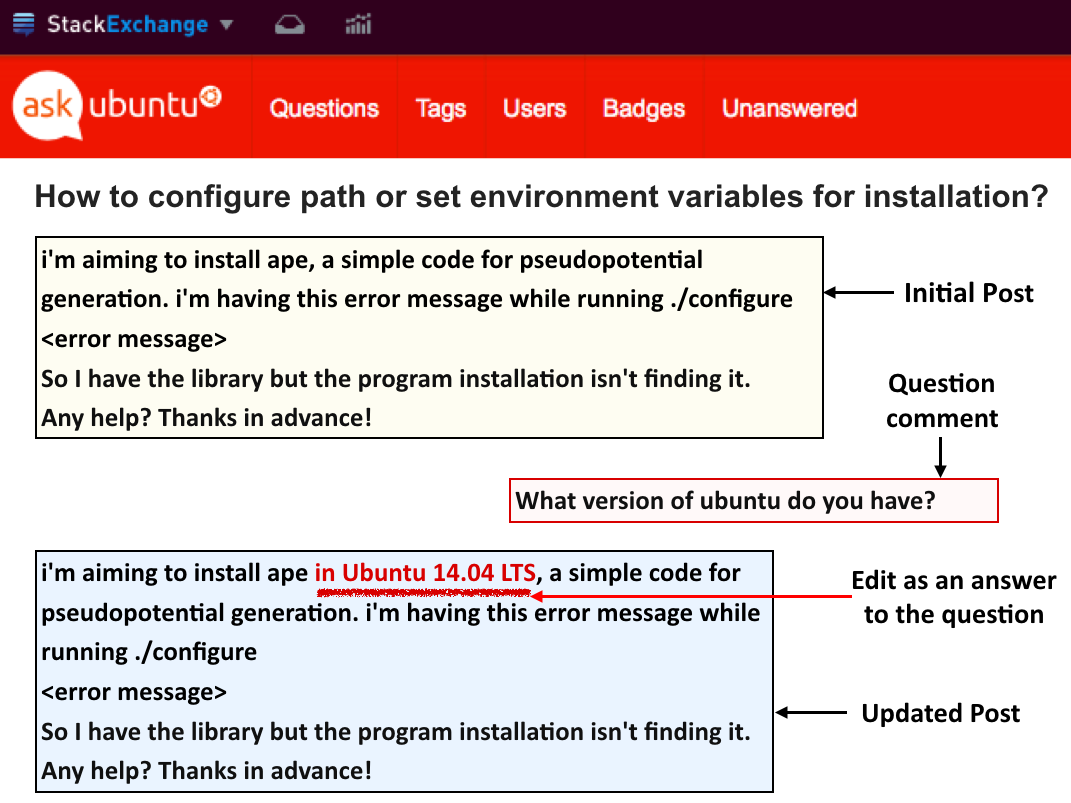
\includegraphics[width=0.47\textwidth]{askubuntu_post}}
	\caption{A post on an online Q \& A forum ``askubuntu.com'' is updated to fill the missing information pointed out by the question comment}
	\label{askubuntu_post}
\end{figure}
%
Our work has two main contributions: 
\begin{enumerate}[noitemsep,nolistsep]
	%\item Identifying the problem of generating clarification questions as a problem worth of study, both in its own right and as part of the larger problem of building naturalistic conversational systems. 
	\item A novel neural-network model for addressing this task that integrates the notion of expected value of perfect information (\S\ref{model}). % , a classic formalization from AI
	\item A novel dataset, derived from StackExchange, that enables us to learn a model to ask clarifying questions by looking at the types of questions people ask (\S\ref{dataset_creation}).\footnote{We use data from StackExchange; per license cc-by-sa 3.0, the data is ``intended to be shared and remixed'' (with attribution). We will release all of the data we extract.}
\end{enumerate}

To develop our model we take inspiration from the decision theoretic framework of the Expected Value of Perfect Information (EVPI), a measure of the value of gathering additional information. In our setting, we use EVPI to calculate which question is most likely to elicit an answer that would make the post more informative.
Formally, for an input post $p$, we want to choose a question $q$ that maximizes $\mathbb{E}_{a \sim p,q}[\U(p+a)]$, where $a$ is a hypothetical answer and $U$ is a utility function measuring the \emph{completeness} of post $p$ if $a$ were to be added to it.
To achieve this, we construct two models:
(1) an answer model, which estimates $\mathbb{P}[a~|~p,q]$, the likelihood of receiving answer $a$ if one were to ask question $q$ on post $p$;
(2) a completeness model, $\U(p)$, which measures how complete a post is.
Given these two models, at prediction time we search over a shortlist of possible questions for that which maximizes the EVPI.

We are able to train these models jointly based on $(p,q,a)$ triples that we extract automatically from StackExchange.
Figure~\ref{askubuntu_post} depicts how we do this using StackExchange's edit history.  In the figure, the initial post fails to state what version of Ubuntu is being run. In response to Parker's question in the comments section, Terry, the author of the post, edits the post to answer Parker's clarification question. We extract the initial post as $p$, question posted in the comments section as $q$, and edit to the original post as answer $a$ to form our $(p,q,a)$ triples. 

Our results show significant improvements from using the EVPI formalism over both standard feedforward network architectures and bag-of-ngrams baselines, even when our system builds on strong information retrieval scaffolding. In comparison, without this scaffolding, the bag-of-ngrams model outperforms the feedforward network. We additionally analyze the difficulty of this task for non-expert humans, and give examples of system output. %on which our system does well, and several on which it does poorly.


%Questions posted in the comments section often times include possible solutions or suggestions phrased as a rhetorical question. To filter out such non-clarification questions, we further train a classifier on a small set of questions labelled as clarification/non-clarification using a crowdsourcing platform. We compare the predictions of our model with human judgements obtained on a small held out test set and TODO
% consisting of initial posts $p$, clarification questions in the comments section

%the first estimates, for any hypothetical answer, how much more \emph{complete} the original post would be if this answer were added to it;
%the second estimates, for any fixed question, what is the likelihood of a possible ans
%Figure~\ref{model} depicts the following three components of our EVPI inspired model: 
%\begin{enumerate}
%\item For a given unanswered post $p_i$, we generate a set of question candidates $Q_i$ by looking at questions that were asked to posts similar to the unanswered post $p_i$ %(Section~\ref{candidate_question_generator})
%\item For each of the candidate questions $q_{j} \in Q_i$, we generate an answer representation $a_{j}$ given the unanswered post  $p_i$ and the candidate question $q_{j}$ %(Section~\ref{answer_generator})
%\item Finally we calculate the utility of each of the updated posts $(p_i + a_{j})$ and output the question that maximized the utility of the updated post %(Section~\ref{utility_calculator})
%\end{enumerate}

% Our model for $\mathbb{P}[a~|~p,q]$ takes the text of a post $p$ and an answer $q$ and runs them through LSTMs to obtain a single embedding.
% Answers $a$ are represented using embeddings and the model is trained to minimize the distance between the answer and the embedding of $(p,q)$.
% The probability model over $a$ then takes the form of a Gaussian centered around the embedding of $(p,q)$.
% Our model for $U(p+a)$ takes an \emph{average} embedding of the sentences in $p$ and the embedding of $a$ and produces an estimate $U(p+a)$ that ranges in $[0,1]$ for how complete this post is.

% In order to train our model, we use two complementary datasets, one for estimating $\mathbb{P}[a~|~p,q]$ and one for estimating $U(p+a)$.
% Although these two components are trained on different datasets, they are trained jointly to optimize an answer selection criterea. TODO is this true?
% To train the answer predictor, we use the \emph{edit history} of StackExchange, as depicted in Figure~\ref{askubuntu_post}. 
% We extract initial posts $p$, questions from the comments section $q$, and answers from edits to the initial post $a$ to form $(p,q,a)$ triples.
% To train the completeness predictor, we can use a much larger dataset comprised of posts-which-eventually-get-answers (positive examples for completeness) and posts-which-remain-unanswered (negative examples).
% Although this labeling is noisy, \newcite{asaduzzaman2013answering} suggest that a primary reason that StackExchange posts remain unanswered is due to incompleteness.

%We train our model using a neural network framework to minimize an objective function defined using EVPI. We compare our model with a bag-of-words baseline and a neural baseline; both which are trained to select the right question given a post and question candidates; without generating an answer for the question. Human judgements on a held out test set of unanswered posts show that our EVPI inspired model can learn to ask questions better.

%We can mine many (post, question, answer) triples from StackExchange's edit histories. In the figure, the initial post fails to state what version of Ubuntu is being run. A person then asked for the Ubuntu version in the comments section. Next, the original poster edited their post, answering the clarification question. Based on this data, we will learn how to choose what question would be most useful to ask. A good question is one whose answer is most likely to help someone respond to the initial request, a notion captured in the theory of expected value of perfect information.


%\iffalse
%-- we show that we can train two different models when we have varied amount of training data? (ask Hal)
%\fi

\begin{figure*}[t]
	\centering
	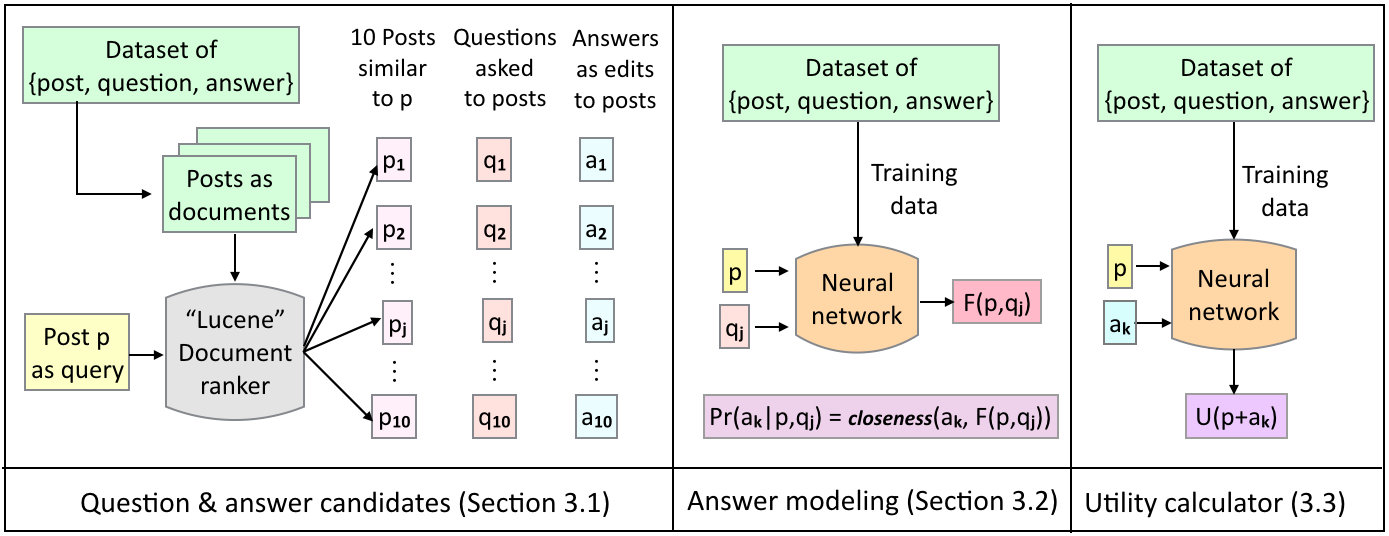
\includegraphics[width=0.85\textwidth]{model}
	\caption{\small The behavior of our model during test time. Given a post $p$, Lucene retrieves 9 posts similar to post $p$ and consider the questions asked to those 9 posts, plus the original, as question candidates. The edits made to the posts in response to the questions as our answer candidates. For each question candidate $q_i$, we generate an answer representation $F(p,q_j)$ and calculate how close is the answer candidate $a_k$ to our answer representation $F(p,q_j)$. Our utility calculator calculates the utility of the post if it were updated with the answer $a_k$. Finally we return the question $q$ that maximizes the expected utility of the post $p$ (Equation~\ref{evpi_equation}).}
	\label{model}
\end{figure*}

\section{Related Work} \label{related_work}

The problem of question generation has received sparse attention from the natural language processing community. Most prior work focuses on generating reading comprehension questions:  given text, write questions that one might find on a standardized test \cite{vanderwende2008importance,heilman2011automatic,rus2011question,olney2012question}.  Comprehension questions, by definition, are answerable from the provided text. Clarification questions are not.  

Outside reading comprehension questions, \newcite{labutov2015deep} generate high-level question templates by crowdsourcing and given a text segment, rank question templates that are relevant. However the crowdsourcing method of collecting data leads to significantly less data than we collect using our method. \newcite{liu2010automatic} use template question generation to help authors write better related work sections. \newcite{mostafazadeh2016generating} introduce a Visual Question Generation task where they consider question generation from images, a multi-modal variant of question generation. 
\newcite{penas2010filling} identify the notion of missing information similar to us but they attempt to fill the knowledge gaps in a text with the help of external knowledge bases, whereas we instead ask clarification questions. \newcite{artzi2011bootstrapping} use human-generated clarification questions to drive a semantic parser where the clarification questions are aimed towards simplifying a user query; whereas we generate clarification questions aimed at  identifying missing information in a text. 

%The problem of question generation has received sparse attention from the natural language processing community. In fact, we know of no work that addresses the problem of generating clarification questions. Most prior work has focused on generating reading comprehension questions \cite{vanderwende2008importance,penas2010filling,heilman2011automatic,olney2012question}: given text, write comprehension questions that one might find on a standardized test. Comprehension questions, by definition, are answerable from the provided text. Clarification questions are not. 
%
%Outside reading comprehension questions, \newcite{labutov2015deep} studied the problem of generating question templates via crowdsourcing, which leads to significantly less data that we can collect. \newcite{liu2010automatic} use template question generation to help authors write better related work sections. \newcite{mostafazadeh2016generating} consider question generation from images, which may or may not be clarifications TODO note we don't guarantee ours are clarification either :P. \newcite{artzi2011bootstrapping} use human-generated clarification questions to drive a semantic parser.

\section{Model description}\label{model}

In order to choose what question to ask, we build a neural network model inspired by the theory of expected value of perfect information (EVPI). EVPI is a measurement of: if I were to acquire information X, how useful would that be to me? However, because we haven't acquired X yet, we have to take this quantity in expectation over all possible X, weighted by each X's likelihood. In the question generation setting, for any given question $q$ that we can ask, there is set $A$ of possible answers that could be given. For each possible answer $a \in A$, there is some probability of getting that answer, and some utility if that were the answer we got. The value of this question $q$ is the expected utility, over all possible answers. The theory of EVPI then states that we want to choose the question $q$ that maximizes:
\begin{equation}\label{evpi_equation}
\argmax_{q \in Q} \sum_{a \in A} \mathbb{P}[a | p,q] \U(p+a)
\end{equation} 

In Eq~\ref{evpi_equation}, $p$ is the post, $q$ is a potential question from a set of candidate questions $Q$ and $a$ is a potential answer from a set of candidate questions $A$. $\mathbb{P}[a | p,q]$ measures the probability of getting an answer $a$ given an initial post $p$ and a clarifying question $q$. $\U(p+a)$ is a utility function that measures how useful it would be if $p$ were augmented with answer $a$. In our case, the utility function we use is the completeness of the post: a post has high utility the more complete it is. This captures the right intuition in the example questions (from Section~\ref{introduction}) that Parker could have asked such that: \textsf{\small (a)} will have good utility for many likely answers;
\textsf{\small (b)} will have low utility regardless of the answer; and
\textsf{\small (c)} will have high utility only for a low probability answer.

The modeling question then is how to model: 
%\begin{enumerate}[noitemsep,nolistsep]
(1) the probability distribution $\mathbb{P}[a | p,q]$ and
(2) the utility/completeness function $\U(p+a)$.
In our work, both will be represented using neural networks over the appropriate inputs. Posts, questions and answers will all be represented as embeddings. We train the parameters of the two models jointly to minimize a joint loss defined such that an answer that has a higher potential of increasing the utility of a post gets a higher probability.

Figure~\ref{model} describes the behavior of our model during test time. 
Given a post $p$, our first step is to generate a set of candidate questions and a set of candidate answers (Section~\ref{question_candidate_generator}).
Given a post $p$ and a question candidate $q_i$, our second step is to calculate how likely is this question to be answered using one of our answer candidates $a_k$ (Section~\ref{answer_modeling}).
Given a post $p$ and an answer candidate $a_k$, the third step is to calculate the utility of the updated post i.e. $\U(p + a_k)$ (Section~\ref{utility_calculator})
Finally, using these pieces, we build a joint neural network that we can optimize end-to-end over our data (Section~\ref{neural_network}).

\subsection{Question \& answer candidate generator}\label{question_candidate_generator}

Given a post $p$, our first step is to generate a set of candidate questions and a set of candidate answers. One way that humans learn to ask questions is by looking at how others ask questions in a similar situation. Using this intuition we generate question candidates for a given post by identifying posts similar to the given post and then looking at the questions asked to those posts. For identifying similar posts, we use Lucene\footnote{\url{https://lucene.apache.org/}}, a software extensively used in information retrieval for extracting documents relevant to a given query from a pool of documents. Lucene also ranks the extracted documents according to their relevance to the query. We use Lucene to find the top 10 most similar posts to a given post from our dataset (Section~\ref{dataset_creation}) \footnote{The top most similar candidate to a post is the original post itself}. We consider the questions asked to these 10 posts as our set of question candidates and the edits made to the posts in response to the questions as our set of answer candidates. Section~\ref{dataset_creation} describes the process of extracting the (\textit{post, question, answer}) triples from the StackExchange datadump. 

\begin{figure*}[ht]
	\centering
	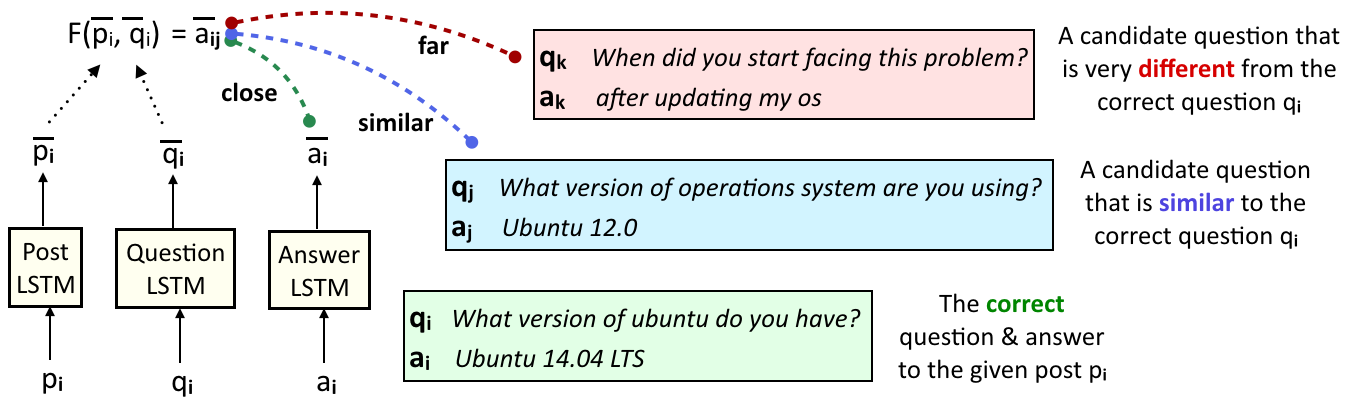
\includegraphics[width=0.9\textwidth]{answer_generator}
	\caption{Training of our answer generator. Given a post $p_i$ and its question $q_i$, we generate an answer representation that is not only close to its correct answer $a_i$, but also close to one of its candidate answers $a_j$ if the candidate question $q_j$ is close to the true question $q_i$.}
	\label{fig_answer_generator}
\end{figure*}

\subsection{Answer modeling}\label{answer_modeling}

Given a post $p$ and a question candidate $q_i$, our second step is to calculate how likely is this question to be answered using one of our answer candidates $a_k$. To calculate this probability, we first generate an answer representation using $p$ and $q_i$ and then measure how close is the answer candidate $a_k$ to our answer representation. To model our answer generator we use the following intuition: a question can be asked in several different ways. For e.g. in Figure~\ref{askubuntu_post}, the question ``\textsf{\small What version of Ubuntu do you have?}'' can be asked in other ways like ``\textsf{\small What version of operating system are you using?}'', ``\textsf{\small Version of OS?}", etc.  
Additionally, for a given post and a question, there can be several different answers to that question. For instance, ``\textsf{\small Ubuntu 14.04 LTS}", ``\textsf{\small Ubuntu 12.0}", ``\textsf{\small Ubuntu 9.0}", are all valid answers. We train our answer generator to generate an answer representation capturing these generalizations.

We use our dataset of \{\textit{post, question, answer}\} triples (Section~\ref{dataset_creation}). Given a $\{p_i, q_i, a_i\}$ triple, we use a long short-term memory architecture (LSTM) \cite{hochreiter1997long} to get to their respective neural hidden representations $\{\bar p_i, \bar q_i, \bar a_i\}$.  Given $(\bar p_i, \bar q_i)$, we define a feed-forward neural network $F$ that combines the post and question representations to get an answer representation $F(\bar p_i, \bar q_i)$. We train our answer generator to minimize the loss function below:
%
\begin{align}\label{eq_answer_generator}
\textrm{loss}_{\textrm{ans}}(\bar p, \bar q, \bar a, Q) 
&=  {|| F(\bar p, \bar q) - \bar a||}^2 & \\
&\hspace{-25mm} +  \sum_{j \in Q} \Big ( {|| F(\bar p, \bar q) - \bar{a_j} ||}^2  (1 - \tanh{(|| \bar q - \bar{q_j} ||^2)}) \Big ) \Big \} &\nonumber
\end{align}
%
This loss function can be explained using the example in figure~\ref{fig_answer_generator}. Question $q_i$ is the question paired with the given post $p_i$. In equation~\ref{eq_answer_generator}, the first term forces the function $F(\bar p_i, \bar q_i)$ to generate an answer representation as close as possible to the correct answer $a_i$. Now, a question can be asked in several different ways. Let $Q_i$ be the set of candidate questions for post $p_i$, retrieved from the dataset using Lucene (Section~\ref{question_candidate_generator}). Suppose a question candidate $q_j$ is very similar to the correct question $q_i$ ( i.e. $|| \bar q_i - \bar{q_j} ||$ is near zero). Then the second term forces the answer representation $F(\bar p_i, \bar q_i)$ to be close to the answer $a_j$ corresponding to the question $q_j$ as well. Thus in the figure~\ref{fig_answer_generator}, the answer representation will be close to $a_j$ (since $q_j$ is similar to $q_i$), but far off from $a_k$ (since $q_k$ is dissimilar to $q_i$).

Given such an answer representation, we then define the probability distribution over candidate answers $a_k \in A$ as: 
\begin{align}
\mathbb{P}[a_k |p_i,q_j]  
&= \frac 1 Z \exp\left[- \lambda || a_k  -  F(p_i,q_j) ||^2\right]
\end{align}
where $\lambda$ is a tunable parameter that controls the variance of the distribution.

\subsection{Utility calculator}\label{utility_calculator}
Given a post $p$ and an answer candidate $a_k$, the third step is to calculate the utility of the updated post i.e. $\U(p + a_k)$. As expressed in equation~\ref{evpi_equation}, this utility function measures how useful it would be if a given post $p$ were augmented with an answer $a_k$. We train our utility calculator using our dataset of \{\textit{post, question, answer}\} triples (Section~\ref{dataset_creation}). We label all the $(p_i, a_i)$ pairs from our triples dataset with label $y=1$. To get negative samples, we make use of the answer candidates generated using Lucene as described in Section~\ref{question_candidate_generator}. For each $a_k \in A_i$, where $A_i$ is the set of answer candidates for post $p_i$, we label the pair $(p_i, a_k)$ with label $y=0$, except for when $a_k == a_i$. Thus, corresponding to each post $p_i$ in our triples dataset, we get one positive sample and nine negative samples. 

Given a post $p$ and an answer $a$, we use a post LSTM and an answer LSTM to get the neural representation $\bar{p}$ and $\bar{a}$. We define a feedforward neural network that combines the post neural representation $\bar{p}$ and the answer neural representation $\bar{a}$ to get the updated post representation $F(\bar{p}, \bar{a})$. The utility of the updated post is then defined as $\U(p+a) = \sigma ( F(\bar{p}, \bar{a}) )$. We want this utility to be close to 1 for all the positively labelled $(p,a)$ pairs and close to 0 for all the negatively labelled $(p, a)$ pairs. We therefore define our loss using the binary cross-entropy formulation below:
%
\begin{align}\label{eq_utility_calculator}
\textrm{loss}_{\textrm{util}}(y, \bar p, \bar a) &= y \log(\sigma (F(\bar{p}, \bar{a})))
\end{align}

\subsection{Our joint neural network model}\label{neural_network}
Our fundamental representation is based on recurrent neural networks over word embeddings. We obtain the word embeddings using a GloVe \cite{pennington2014glove} model trained on the entire datadump of StackExchange. Given an initial post $p$, we generate a post neural representation $\bar{p}$ using a post LSTM i.e. long short-term memory architecture \cite{hochreiter1997long} as shown in the figure~\ref{lstm}. Similarly, given a question $q$ and an answer $a$, we generate a question neural representation $\bar{q}$ and a answer neural representation $\bar{a}$ using a question LSTM and an answer LSTM respectively. We define the function $F$ as a feedforward neural network on its input with two fully-connected hidden layers. So the function $F(\bar{p},\bar{q})$ in our answer model would be a feedforward neural network on the inputs $\bar{p}$ and $\bar{q}$ and the function $F(\bar{p}, \bar{a})$ in our utility calculator would be a feedforward neural network on the inputs $\bar{p}$ and $\bar{a}$. We train the parameters of the three LSTMs corresponding to $p$, $q$ and $a$, and the parameters of the two feedforward neural networks jointly to minimize the sum of the loss of our answer model (Eq~\ref{eq_answer_generator}) and our utility calculator (Eq~\ref{eq_utility_calculator}):
%
\begin{align}
\sum_i \textrm{loss}_{\textrm{ans}}(\bar p_i, \bar q_i, \bar a_i, Q_i)  
+  \textrm{loss}_{\textrm{util}}(y_i, \bar p_i, \bar a_i)
\end{align}
%
Given such an estimate $\mathbb{P}[a|p,q]$ of an answer and a utility $\U(p+a)$ of the updated post, predictions (i.e., selecting a question from a set of candidate questions) can be done by choosing that ``$q$'' that maximizes Eq~\ref{evpi_equation}. The remaining question, then, is how to get data that enables us to train our answer model and our utility calculator. Given data, the training becomes a multitask learning problem, where we learn simultaneously to predict utility and to estimate the probability of answers.

\begin{figure}
	\centering
	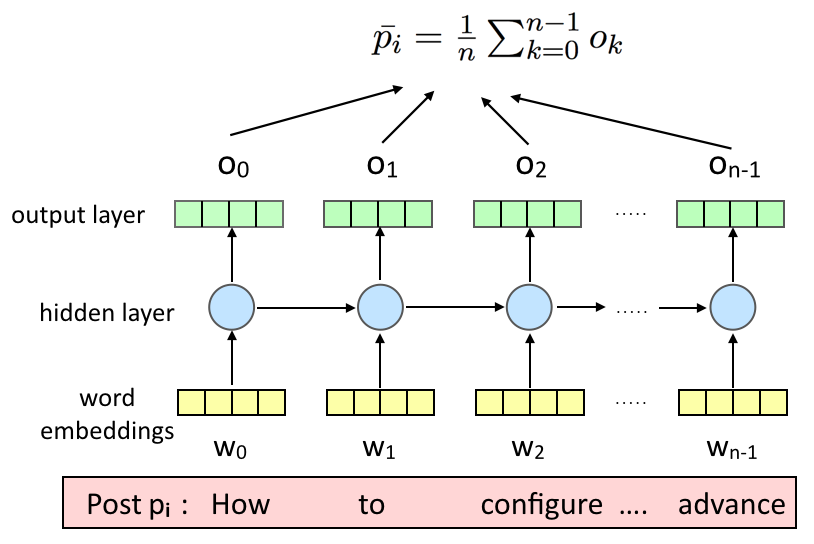
\includegraphics[scale=0.27]{lstm}
	\caption{{\small Our LSTM architecture on a post $p_i$. The input layer consists of pre-trained word embeddings of the words in the post which is fed into a single hidden layer. The output $o_k$ of each of the hidden states is averaged together to get our neural representation $\bar p_i$}}
	\label{lstm}
\end{figure}

\section{Dataset creation}\label{dataset_creation}
StackExchange is a network of online question answering websites about varied topics like academia, ubuntu operating system, latex, etc. The sites are modeled after StackOverflow, a popular platform used for asking and answering questions on a wide range of topics in computer programming. The data dump of StackExchange contains timestamped information about the posts, comments on the post and the history of the revisions made to the post. We use this data dump to create our dataset of \{\textit{post, question, answer}\} triples: where the \textit{post} is the initial unedited post, the \textit{question} is the comment containing a question and the \textit{answer} is the edit made to the post that matches the question comment. \\
\textbf{Extract posts:} We use the post histories to identify posts that have been updated by its author. We use the timestamp information to retrieve the initial unedited version of the post.\\
\textbf{Extract questions:} For each such initial version of the post, we use the timestamp information of its comments to identify the first comment made to the post. We look for a question mark `?' token to further identify if its a question comment. Finally, we truncate the comment till the question mark token to retrieve the question part of the comment.\\
\textbf{Extract answers:} In our final step, we identify the edit made to the post in response to the question comment. Authors make edits to their posts for several reasons; including stylistic updates and grammatical corrections. Therefore, we use only those edits that are longer than four words and finally use the timestamp information of the edit to match the edits to their respective question comments.

%We extract a total of 38,041 (\textit{post, question, answer}) triples from StackExchange which are distributed across three domains: askubuntu (13,749), unix (6656), and superuser (17,636). We train our models using 80\% of the data, tune our hyper parameters using 10\% of the data and evaluate our models using the remaining 10\% of the data. Table~\ref{data_statistics} shows the sizes of the train, dev and test splits for the three domains. 
\begin{table}
	\centering
	\begin{tabular}{lccc}
		\toprule
		& Train & Dev & Test  \\
		\midrule
		askubuntu & 10,992 & 1374 & 1375\\
		unix & ~~~5324 & ~~666 & ~~666 \\
		superuser & 14,828 & 1404 & 1404 \\
		\bottomrule
	\end{tabular}
	\label{data_statistics}
	\caption{Table above shows the sizes of the train, dev and test split of our dataset for three domains.}
\end{table}

A natural question to our process of data creation would be how often is the extracted question a clarification question. We sample a set of 1400 questions from our dataset and design a crowdsourced task where given a question we ask a human to choose whether: a) It is a clarification question, b) It provides an answer or a suggestion; or c) Neither.  63\% of the questions are marked as clarification question, 33\% of them are marked as questions that provides an answer or a suggestion and 4\% of them are marked as neither. The inter-annotator agreement (PAA) is above 90\%. These numbers suggest that although a greater percentage of the extracted questions are clarification questions, our data is imperfect: it includes some non-clarification questions.

\section{Experimental Results}\label{experiments_results}
Our primary research questions that we evaluate experimentally are:
%
\begin{enumerate}[noitemsep,nolistsep]
	\item Does a neural architecture with learned representations improve upon a simple bag-of-ngrams baseline?
	
	\item Does the expected value of perfect information (EVPI) formalism provide leverage over a similarly expressive feed-forward network? %In particular, is EVPI a useful inductive bias for a model?
	
	\item In the EVPI formulation, is it useful to compute an expectation over answers, rather than just picking a single question/answer pair?
	
	\item How well does our model perform in comparison to non-expert humans?
	
	\item How much harder is the task when the (distrator) candidate questions come from Lucene rather than selected randomly?\footnote{A common strategy with the Ubuntu dialogue corpus \cite{lowe2015ubuntu} is to train a dialogue system by choosing a best response given a context of a conversation and a set of candidate responses. However, these methods generate their candidates from their dataset using random sampling. This plausibly makes the task significantly easier than using Lucene to select candidates, which are much more likely to be confusable and have high lexical overlap.}
\end{enumerate}

% In contrast, we generate our candidates using Lucene, a well-known information retrieval system, and so our candidate questions are more closer to each other than a randomly sampled questions would have been. Thus, we indirectly define a harder task. To compare how our models perform in an easier configuration, we design our experiments on two task setups (Section~\ref{task_setup}). To understand the leverage our EVPI inspired model gets us, we compare our model with non-neural baselines and feedforward neural baselines (Section~\ref{baselines}). 

% Further, we design another experiment where in equation~\ref{evpi_equation}, instead of choosing the question that maximizes the expected utility over all possible answers (EVPI max), we choose the question whose answer has the maximum utility (EVPI sum). This experiment helps us understand the leverage we are getting by summing over all our answer candidates, further strengthening the case for our EVPI inspired model. 

\begin{table*}[t]
	\small
	\centering
	\begin{tabular}{l|cccc|cccc}
		\toprule
		& \multicolumn{4}{c|}{Lucene negative candidates} & \multicolumn{4}{c}{Random negative candidates} \\
		Models & Acc & MRR & R@3 & R@5 & Acc & MRR & R@3 & R@5\\
		\midrule
		Random  & 10.0 & 29.3 & 30.0 & 50.0 &10.0 & 29.3 & 30.0 & 50.0 \\
		Bag-of-ngrams & 11.6 & 31.3 & 32.5 & 54.6 & 54.9 & 70.5 & 83.1 & 92.0 \\
		Feed-forward & 17.4 & 37.8 & 43.2 & 63.9 &  49.0 & 66.8 & 81.3 & 92.8 \\
		EVPI max  & 21.1 & 41.2 & 48.0 & 66.9  & 48.8 & 65.5 & 77.2 & 89.9 \\
		EVPI sum & \bf 23.3 & \bf 43.4 & \bf 51.0 & \bf 70.3 & \bf 61.1 & \bf 75.5 & \bf 87.9  & \bf 95.8  \\
		\bottomrule
	\end{tabular}
	\label{results_topN}
	\caption{Results of our two setups `Lucene negative candidates' and `Random negative candidates' on askubuntu test split when the model is trained on a combination of askubuntu, unix and superuser train splits}
\end{table*}


\subsection{Task setups}\label{task_setup}

\textbf{Lucene negative candidates:} In this setup, given a post $p$, we label the question $q$ paired with $p$ in our dataset of $(p, q, a)$ triples as positive. To get our negative candidates, we retrieve nine additional question candidates using Lucene (as described in Section~\ref{question_candidate_generator}).\\
\textbf{Random negative candidates:} In this setup, given a post $p$, we label the question $q$ paired with $p$ in our dataset of $(p, q, a)$ triples as positive as in the previous setting. To get our negative candidates, we randomly sample nine other questions from our dataset of $(p, q, a)$ triples.\footnote{In all cases we train 100-d word embeddings using GloVe \cite{pennington2014glove} on the 3 billion token datadump of StackExchange. We use a threshold frequency of 100 to create our vocabulary of ~250,000 tokens. For our feed-forward neural network, we use two fully-connected dense hidden layers each of size 100. We use ReLU \cite{nair2010rectified} non-linearity as our activation function between the hidden layers.}


\subsection{Baseline methods}\label{baselines}

We compare our model with the following baselines:\\
\textbf{Random baseline:} Given a post, we randomly permute its set of 10 candidate questions uniformly.\\
\textbf{Bag-of-ngrams baseline:} Given a post and a set of 10 question question and answer candidates, we construct a bag-of-ngrams representation for the post, the question and the answer. Our bag-of-ngrams baseline is then trained to minimize hinge loss on misclassification loss using cross-product features between each of (\textit{post, question}), (\textit{question, answer}) and (\textit{post, answer}). We tune the ngram length and the learning rate and choose the setting that performs best on development data.\\
\textbf{Neural network baseline using post, question and answer:} We concatenate the post LSTM representation, the question LSTM representation and the answer LSTM representation and feed it through a feed forward neural network of two fully-connected hidden layers to get our neural baseline. 

\subsection{Dataset}\label{dataset}
We evaluate our model and our baselines on the following three domains of StackExchange: askubuntu, unix and superuser.
% \begin{description}
% \item[askubuntu:]  A question and answer site for users of the Ubuntu Operating system where people post queries about issues they face while using Ubuntu. An example question on this site: ``\textsf{\small Why isn't Chromium up-to-date in all the Ubuntu LTS repos, like Firefox is?}''
% \item[unix:]  A question and answer site for users of Linux, FreeBSD and other unix-like operating systems. This site would contain questions like the ones in askubuntu and more. An example question on this site: ``\textsf{\small How to repeatedly alternate between two (or more) commands?}''
% \item[superuser:] A question and answer site for users of all kinds of operating systems and computer applications. An example question on this site: ``\textsf{\small What is the LAST version of Windows Operating system that can run DOS applications natively?}''
% \end{description}
%
Table~\ref{data_statistics} shows the data statistics for the four sites above.  Although StackExchange consists of many sites, we choose the ones above because: a) The data dump available for them were moderately big in size to train a model on; b) These domains contain clarifications questions that are generic enough to be useful for many different posts; and finally c) The three domains were close enough so that we could combine them to create our full dataset of ~37K triples.

%\subsection{Experimental details}

%\paragraph{Preprocessing:} Each post, question and answer in our dataset of $(post, question, answer)$ triples is represented using embeddings. To generate these embeddings, we first tokenize the raw text in our post, question and answer. We restrict our post to be just the first 100 tokens of the post and our question and answer to be first 10 of their tokens respectively. Given these tokens we then use our word embeddings model to generate their embeddings.

%\paragraph{Word embedding model:} We train 100 dimensional word embeddings using GloVe \cite{pennington2014glove} on the 3 billion token datadump of StackExchange. We use a threshold frequency of 100 to create our vocabulary of ~250,000 tokens. 
%We then train a GloVe model on the datadump to get embeddings of size 100 for each token in our vocabulary. All tokens with a frequency of less than 100 in our dataset get assigned an `UNK'  token.

%\paragraph{Model hyperparameters:}  For our feed-forward neural network, we use two fully-connected dense hidden layers each of size 100. We use ReLU \cite{nair2010rectified} non-linearity as our activation function between the hidden layers. 

\subsection{Results}

We first describe results on the union of all data, summarized in Table~\ref{results_topN}.
We report four metrics: accuracy (percent of time the top ranked question was correct),
mean reciprocal rank (the reciprocal of the ranked position in the top ten list that the correct question is), 
recall at 3 (percent of the the correct answer is in the top three) and
at 5.

The left half of this table shows results when the candidate sets is from Lucene---the ``hard'' setting.
Here, we see that for all the evaluation metrics:
EVPI using the sum (expectation over $a$) outperforms
EVPI using the max $a$;
which outperforms the neural feedforward model that does not incorporate the EVPI formalism;
which outperforms the bag-of-ngrams baseline;
which outperforms the random baseline.
The gains in all cases are relatively large: at least a few percentage points.
A final performance of 51\% recall at 3 is encouraging, though clearly there is a long way to go for a perfect system.

The right half of this table shows the same results when the candidate set is chosen randomly---the ``easy'' setting.
A major difference in the results here is that the bag-of-ngrams system now \emph{outperforms} both the feedforward neural model and the EVPI using max instead of expectation.
This likely happens because just picking up on word overlap---when Lucene has not already done this for us---works remarkably well.
Nonetheless, in all of the metrics, the true EVPI model outperforms all the baselines, achieving at least a 3\% gain over the bag-of-ngrams baseline.

In Table~\ref{results_topM} (supplementary materials), we show results when we work not with the union of all the data, but with each data set individually.
%The top half is against Lucene candidate, the bottom half is against random candidates.
The main observation is that the trends are essentially the same as before: for Lucene negative candidates, bag-of-ngrams underperforms feedfoward, which underperforms EVPI.
This happens because more data helps, and these three domains are sufficiently similar that the additional data---even if it is slightly domain mismatched---is better than nothing.
%The second observation is that the results for EVPI are lower across the board, with the exception of superuser on random negative examples.% (which is sometimes better, sometimes worse).

\subsection{How well can humans do this task?}

In this section we address two natural questions:
(1) how does the performance of our system compare to a human solving the same task?
(2) just because the system selects a question that is not the exact gold standard question, is it certainly wrong?
To answer these questions, we had 14 computer science graduate students perform an annotation task on $50$ examples.
Most of these graduate students are \emph{not} experts in unix or ubuntu, but all are knowledgable.
We provided them with a post and a randomized list of ten possible questions.
They were instructed to select what they thought was the \emph{single} best question to ask, and additionally mark as ``valid'' any additional questions that they thought would also be okay to ask.
We also asked annotators to rate their confidence in $\{0,1,2,3\}$.
Most found this task quite challenging because many of the questions are about subtle nuances of operating system behavior.

These annotator's accuracy on the ``hard'' task of Lucene-selected questions, was only 36\%, significantly better than our best system (23\%), but still far from perfect.
If we limited to those examples on which they were more confident (confidence of 2 or 3), their accuracy raised to 42\%, but never surpassed that.
A major problem for the human annotators is the amount of background knowledge required to solve this problem.
On an easier domain, or with annotators who are truly experts, we might expect these numbers to be higher.

The average number of ``valid'' answers for a single post according to the (admittedly non-expert) annotators was 4.26 (out of ten); the distribution was fairly symmetric and quickly decaying around that number (the median is four).
In the data, 56\% of the examples had at most four options marked as valid; 
28\% had at most 3; 14\% had at most 2; and 6\% had only one valid option (which by definition is also the ``best'' option).
These numbers suggest that an evaluation strategy that takes validity---and not just raw accuracy---is a useful avenue for future research.


\subsection{Example Outputs}

To understand the behavior of the model, we have included five example outputs as supplementary material.
Table~\ref{tab:examples_good} shows two examples in which our model succeeds in selecting the correct question.
In the first, the original poster is asking a question about SSD data and hardware.
The model correctly asks about uefi (the Unified Extensible Firmware Interface, which replaces BIOS), and ranks that output significantly higher than its second guess.
This is particularly impressive since the question mentions neither uefi nor bios. Human annotators said that the third and fifth outputs would also be valid. In the second example, a user is having significant difficulty getting their Ubuntu installation to work, and the model correctly asks about the error of \texttt{\small apt-get install}.
Several other options were marked as valid by annotators in this case as well.

Table~\ref{tab:examples_bad} shows three examples of errors.
In the first example (about sound), the model
completely misses (ranks in last place) the true question about \texttt{\small linux-firmware-nonfree}.
The model instead asks about Pulseaudio, considered a valid question by annotators.
In the second example, the truth is about \texttt{\small apt-get update} but the model instead asked for the ubuntu version (generally a safe bet, and considered valid). %In this case the model fared better and put the correct question in second position.
In the third example, the model asks far too specific a question about \texttt{\small sslstrip-0.9.tar.gz}, rather than the more debugging question which it should have asked about (in position two).
In this case, it's guess was invalid.


\section{Conclusion}

We have described a new dataset for question generation, and attacked this problem from the perspective of question selection.
Our model integrates state-of-the-art neural network structure with the classic notion of expected value of perfect information, which effectively models a pragmatic choice on the part of the questioner: how do I \emph{imagine} the other party would answer if I were to ask this question. Such pragmatic priciples have recently been shown to be useful in other tasks as well \cite{golland2010game,smith2013learning,orita2015discourse,andreas2016reasoning}.

There are three main avenues for improvement of this work.
The first is in evaluation: given that this task is so difficult for humans, but also given that there is no single right question to ask, how can we better measure performance at this task?
This is exactly the same question faced in much research in dialog and generation more broadly \cite{paek2001empirical,lowe2015ubuntu,liu2016not,kannan2017adversarial}.
Second, to make question generation more general, systems need to be able to generalize, for instance by constructing templates of the from ``What version of \_\_\_ are you running?'' into which the system would need to fill a variable. Finally, asking question is a natural component of dialog, and building a collaborative dialog system that can naturally converse with a user is a broad long term goal.

\bibliography{acl2017}
\bibliographystyle{acl_natbib}

\end{document}
